
\documentclass[twocolumn]{article}
\usepackage{hyperref}
\usepackage{enumitem}
\usepackage{graphicx}
\usepackage{amsmath}
\usepackage{mathpazo}
% \usepackage{multicol}
\usepackage[a4paper,
            bindingoffset=0.2in,
            left=1in,
            right=1in,
            top=1in,
            bottom=1in,
            footskip=.25in]{geometry}

\begin{document}
\title{MS Technical Paper: \\ Placement Algorithms for Heterogenous FPGAs}
\author{Brian B Cheng \\ Rutgers University Department of Electrical and Computer Engineering}


\date{}
\maketitle

\section{Keywords}
\begin{itemize}
    \item FPGA, EDA, Placement, Simulated Annealing, Optimization, RapidWright
\end{itemize}


\section{Abstract}
    fdsafdsafdsa.

\section{Introduction}

    Field-Programmable Gate Arrays (FPGAs) have witnessed unprecedented growth in capacity and versatility, driving significant advances in computer-aided design (CAD) and electronic design automation (EDA) methodologies. 
    Since the early-to-mid 2000s, the stagnation of single-processor performance relative to the rapid increase in integrated circuit sizes has led to a design productivity gap, where the computational effort for designing complex chips continues to rise. 
    In FPGA CAD flows—which traditionally encompass logic synthesis, placement, routing, and bitstream generation—the placement stage has emerged as one of the most time-consuming processes. 
    Inefficiencies in placement not only extend design times from hours to days, thereby elevating cost and reducing engineering productivity, but also limit the broader adoption of FPGAs by software engineers who expect compile times akin to those of conventional software compilers. 

    For these reasons, FPGA placement remains a critical research effort even today. 
    In this paper, we study and implement established placement methods by leveraging RapidWright, which is a semi-open-source API that offers backend access to Xilinx's industry-standard FPGA environment, Vivado. 
    We implement multiple variations of simulated annealing placers for Xilinx's 7-series FPGAs, with an emphasis on minimizing total wirelength while mitigating runtime. 
    Our implementation is organized into three consecutive substages. 
    The \textbf{prepacking} stage involves traversing a raw EDIF netlist to identify recurring cell patterns—such as CARRY chains, DSP cascades, and LUT-FF pairs—that are critical for efficient mapping and legalization. 
    In the subsequent \textbf{packing} stage, these identified patterns, along with any remaining loose cells, are consolidated into SiteInst objects that encapsulate the FPGA’s discrete resource constraints and architectural nuances. 
    Finally, the \textbf{placement} stage employs a simulated annealing (SA) algorithm to optimally assign SiteInst objects to physical sites, aiming to minimize total wirelength while adhering to the constraints of the 7-series architecture. 

    Simulated annealing iteratively swaps placement objects guided by a cost function that decides which swaps should be accepted or rejected. 
    Hill climbing is permitted by occasionally accepting moves that increase cost, in hope that such swaps may later lead to a better final solution. 
    SA remains a popular approach in FPGA placement research due to its simplicity and robustness in handling the discrete architectural constraints of FPGA devices. 
    While SA yields surprisingly good results given relatively simple rules, it is ultimately a heuristic and stochastic approach that explores the vast placement space by making random moves. 
    Most of these moves will be rejected, meaning that SA must run many iterations, usually hundreds to thousands, to arrive at a desirable solution.

    In the ASIC domain, where placers must handle designs with millions of cells, the SA approach has largely been abandoned in favor of analytical techniques, owing to SA's runtime and poor scalability. Modern FPGA placers have also followed suit, as new legalization strategies allow FPGA placers to leverage traditionally ASIC placement algorithms and adapt them to the discrete constraints of FPGA architectures. 
    While this paper does not present a working analytical placer, it will explore ways to build upon our existing infrastructure (prepacker and packer) to replace SA with AP.





\section{Brief History of FPGA Architecture}
    \begin{figure}
        \centering
        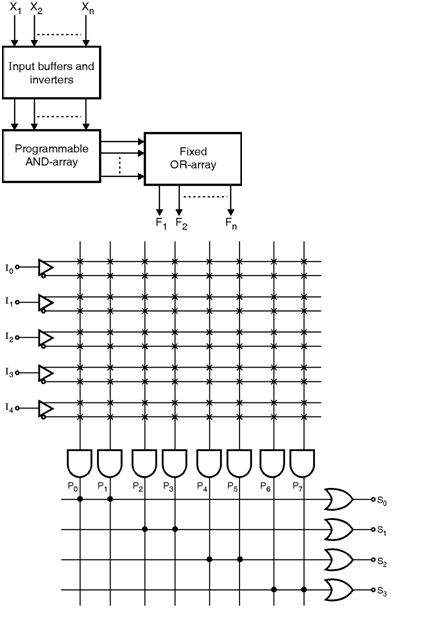
\includegraphics[width=7.0cm]{figures/pal_2.png}
        \caption{PAL architecture with 5 inputs, 8 programmable AND gates and 4 fixed OR gates}
        \label{fig:pla}
        % https://www.electronics-tutorial.net/Programmable-Logic-Device-Architectures/Programmable-Logic-Devices/Programmable-Array-Logic-PAL/
        % https://www.naukri.com/code360/library/difference-between-pla-and-pal 
    \end{figure}

    Before any work can be done on a placer, one must understand the objects being placed and the structure of the medium in which those objects are placed. 
    
    Configurable logic devices have undergone significant evolution over the last four decades.
    The journey began with simple devices like Programmable Logic Array (PLA), which came if the form of logic gates arranged in a "programmable-OR, programmable-AND" plane, used to implement a "sum-of-products" logic equation for each of the outputs in terms of the inputs via programmable fuses. 
    Around the same time came the redundantly named Programmable Array Logic (PAL), which simplified the PLA by fixing the OR gates, resulting in a "fixed-OR, programmable-AND" plane, which sacrificed some flexibility to simplify its manufacture and broaden its applications.

    \begin{figure}
        \centering
        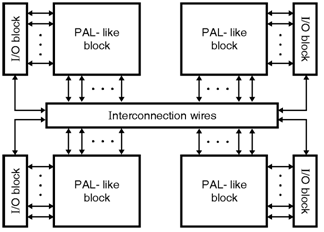
\includegraphics[width=7.0cm]{figures/cpld.png}
        \caption{CPLD architecture with 4 CLBs}
        \label{fig:cpld}
        % https://www.electronics-tutorial.net/Programmable-Logic-Device-Architectures/CPLD/Complex-Programmable-Logic-Device-CPLDs/
    \end{figure}


    Then came the Complex Programmable Logic Device (CPLD), which came as an array of Configurable Logic Blocks (CLBs) stitched together by interconnection wires.
    These CLBs usually took the form of modified PAL blocks, which contained the PAL itself and some macrocells including flip-flops, multiplexers, and tri-state buffers.
    The CPLD was essentially an array of PALs interconnected by a programmable switch matrix and could be programmed via a hardware description language (HDL) like VHDL.

    \begin{figure}
        \centering
        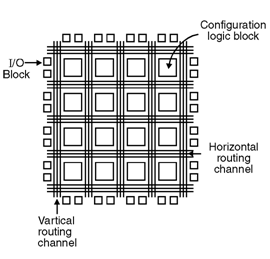
\includegraphics[width=7.0cm]{figures/fpga.png}
        \caption{Island-style FPGA architecture with 16 CLBs}
        \label{fig:fpga}
        % https://www.electronics-tutorial.net/Programmable-Logic-Device-Architectures/FPGA/Field-programmable-gate-array-FPGA/
    \end{figure}




\section{Xilinx 7-Series Architecture}



    \begin{figure*}
        \centering
        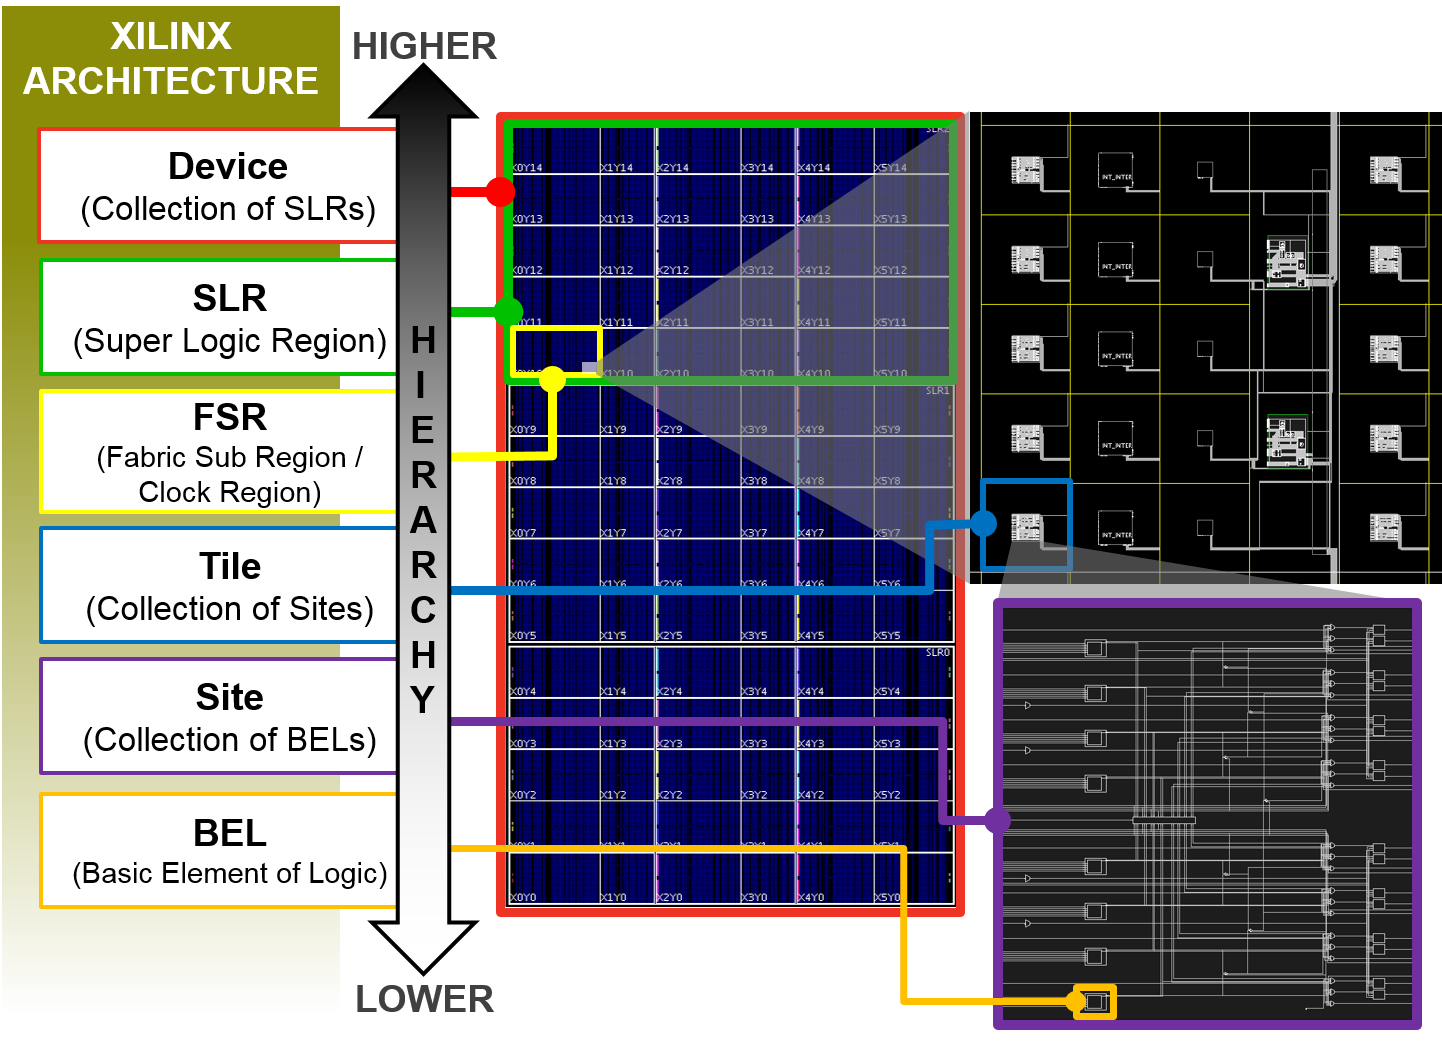
\includegraphics[width=\textwidth]{figures/hierarchy.png}
        \caption{Architecture Hierarchy of a Xilinx FPGA}
        \label{fig:hierarchy}
    \end{figure*}

    Figure~\ref{fig:hierarchy} illustrates the architectural hierarchy of a Xilinx FPGA. 
    At its most basic level, an FPGA is a vast physical array of replicated atomic components known as Basic Elements of Logic (BELs).
    These BELs, which include programmable lookup tables (LUTs), flip flops (FFs), and programmable interconnects, form the fundamental building blocks for custom digital circuit implementations on FPGAs.

    In modern FPGAs like the Xilinx 7-Series, additional BELs like Block RAM (BRAM) and Digital Processing Slices (DSPs) are also available, creating a more heterogeneous programmable logic fabric. 
    These dedicated resources allow designers to implement common digital structures, such as multipliers and memories, without having to recreate them from scratch using only LUTs and flip flops.

    The Xilinx architectural hierarchy organizes these BELs into increasingly abstract structures. 
    \textbf{BELs} are packaged into \textbf{Sites}, which are then embedded into \textbf{Tiles}, which are subsequently consolidated into \textbf{Clock Regions}. 
    In high-end Xilinx devices, Clock Regions may be further consolidated into \textbf{Super Logic Regions} (SLRs). 
    However, for the scope of this paper, we focus on Xilinx devices that have only a single SLR.

    Take for example, the xc7z020 chip, a low-end Xilinx device from the 7-Series family of FPGAs, commonly found on hobbyist boards like the Digilent Arty-Z7.

\section{The FPGA Design Flow and Toolchain}
    \begin{figure}
        \centering
        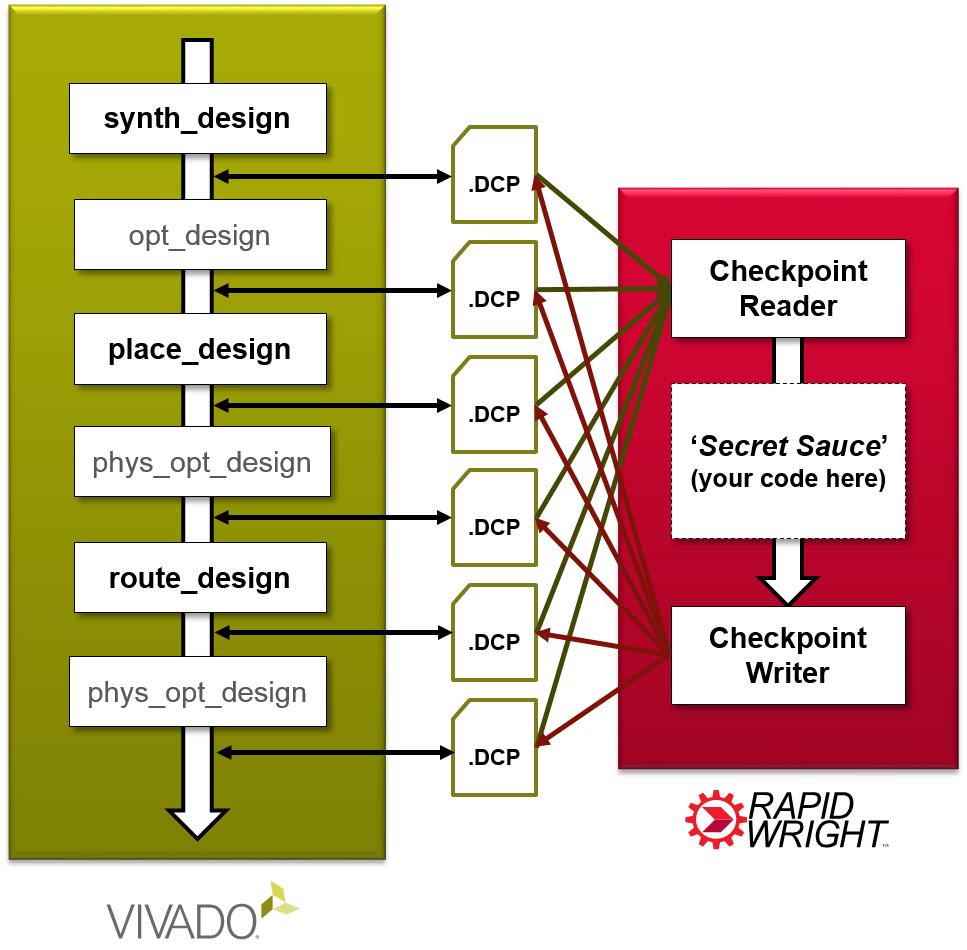
\includegraphics[width=6.5cm]{figures/vivado_dcps.png}
        \caption{Showing how RapidWright can take a design checkpoint at different stages of the Vivado toolchain, make customizations, then feed it back into the toolchain.}
        \label{fig:device_carry_chain_routing}
    \end{figure}
    A typical FPGA design flow goes like the following:
    Engineer design entry (Verilog, VHDL) \\
    Synthesis (Instantiation, substitution, inference, and optimization) \\ 
    Placement (Prepacking, Packing, Global Placement, Legalization, Detailed Placement)\\ 
    Routing \\ 
    Bitstream generation \\ 

\section{RapidWright API}

    DO WE REALLY NEED THIS SECTION? JUST REFERENCE THE RW DOCUMENTATION.

    The RapidWright API offers a user-friendly toolkit to take pre-implemented designs, that is, designs that have already been placed and/or routed by Vivado, and make custom optimizations to fit complex design criteria. 
    RapidWright has several "BlockPlacers", a general Router, but no general Placer. 
    We use this API to implement a crude general placer, in our case, a simulated annealer. 
    (Show what parts of the FPGA toolchain that RapidWright already has and how our placer fits into that toolchain). 

    There are three packages of objects that are most relavent to building our placer: the edif package, design package, and device package.

    \subsection{Device Objects}
    The \textbf{device} package contains the classes that correspond to constructs in the hardware and/or silicon devices. 
    The most prominent class, aptly named Device, represents a specific product family member (like the xc7z020 device of the 7-series family) and provides a reference to all of the logical and routing resources available on the device.
    There device classes can be separated into two groups: logical and routing.
    Among the logical classes are the BEL, Site, Tile, and ClockRegion objects discussed before.
    Among the routing classes are BELPin, SitePin, PIP (Programmable InterConnect Point), Wire, and Node.


    \subsection{Design Package}
    The \textbf{design} package is the collection of objects used to describe how a logical netlist maps to the device netlist. 
    The design is also referred to as the "physical netlist" or "implementation".
    It contains all of the primitive logical cell mappings to hardware, specifically the cells to BEL placements and physical net mapping to programmable interconnect or routing.

    \subsection{EDIF Package}


\section{Placement Implementation}
    (Describe the algorithm, then in context of 7-Series arhictecture). \\
    \subsection{PrePacking}
        In the prepacking stage, we traverse the raw EDIF Netlist to identify recurring cell patterns. In particular, we will specifically look for CARRY chains, DSP cascades, and LUT-FF pairs.
        \subsection{CARRY Chains}
            Each SLICE Site contains one CARRY4 BEL.
            Each CLB Tile contains two SLICE Sites.
            CARRY chains span vertically across multiple SLICE Sites/Tiles. (Show picture)
            \begin{figure}
                \centering
                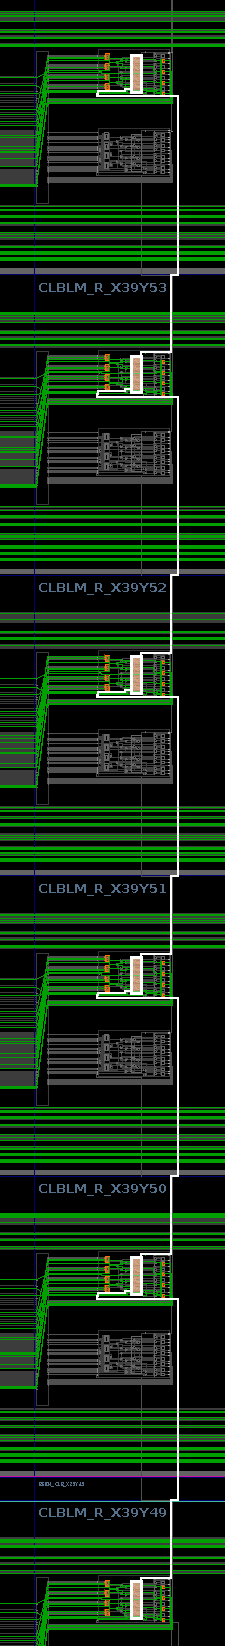
\includegraphics[width=3.0cm]{figures/carry_chain_routes.png}
                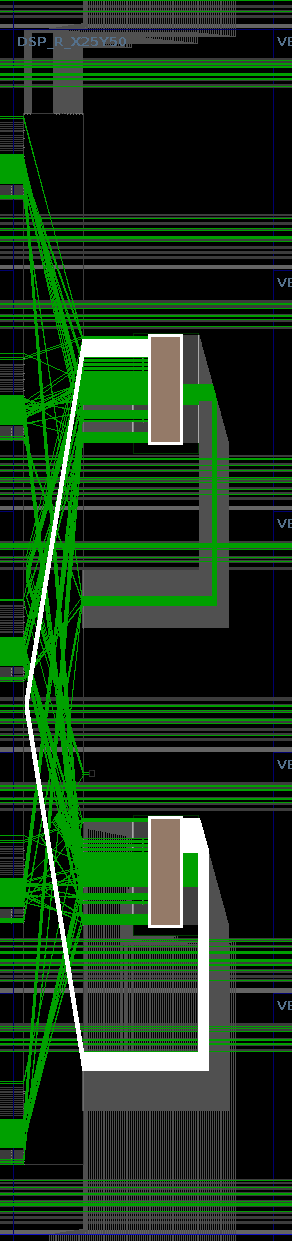
\includegraphics[width=3.0cm]{figures/dsp_cascade_routes.png}
                \caption{A Carry Chain of length 6 spanning 6 Tiles. On the left, the cell-only representation. On the right, cells with routing representation.}
                \label{fig:device_carry_chain_routing}
            \end{figure}
        \subsection{DSP Cascades}
            Each DSP Site contains one DSP BEL.
            Each DSP Tile contains two DSP Sites.
            DSP chains can span vertically across multiple DSP Sites/Tiles.

        \subsection{LUT-FF Pairs}
            Identify unique CE-SR net pairs. All FF cells in a Site must share the same CE and SR nets.
    \subsection{Packing}
        In the packing stage, we take the identified cell clusters and pack them into SiteInst Design objects which target the Device Site objects.
        \subsection{CLB Sites}
            Can support LUT-FF pairs, loose LUTs, loose FFs, CARRY chains.
            Each SLICE has 8 "lanes" of LUT-FFs. 4 LUT5s and 4 LUT6s. 8 FFs.
            For SLICEMs, LUT6s can be configured as shallow 32-bit LUTRAMs or "RAMS32".
    \subsection{Placement}
        Create BEL "fields": CLB, DSP, CLB and DSP Chains, RAMs

        \subsection{Detailed Placement}







\section{Analytical Placement}
    Introduce placement with legalization methods. \\
    Many AP approaches use a Global placement, Legalization, then Detailed placement approach. \\
    Our SA only considers legal moves via bookkeeping structures, so it has no concept of global placement or legalization. \\
    It is a detailed placement only approach. \\
    \begin{itemize}
        \item Talk about HeAP as an example.
        \item Global Placement, Legalization, then Detailed Placement approach.
        \item Global placement using the Bound2Bound net model from SimPL.
        \item Legalization Step 1: \\
            Find an area of the device that is overutilized (illegal) for twhich the blocks contained within must spread to a larger area. \\
            To obtain this overutilized area, adjacent locations (Sites, Tiles, etc.) on the device that are occupied by more than one block (SiteInst, ModuleInst, etc.) are repeatedly clustered together, until all clusters are bordered on all sides by non-overutilized locations. \\ 
            Then, the area (?) is expanded in both the x and y dimensions (?) until it is large enough to accommodate all blocks contained within. \\
            Specifically, the area is expanded until its "occupance" \(O_A\) divided by its "capacity" \(C_A\) is less than a maximum "utilization factor" $\beta$, where $\beta$ is less than or equal to 1. HeAP uses 0.9.
        \item Legalization Step 2: \\
            Two cuts are generated: a "source cut" and a "target cut". \\
            The source cut pertains to the blocks being placed (SiteInsts in home buffer). \\ 
            The target cut pertains to the area into which the blocks are placed (away buffer). \\
            The source cut splits the blocks into 2 partitions, while the target cut splits the area into 2 sub-areas, into which the blocks in each partition are spread. \\
            Two objectives are minimized during this process: The imbalance between the number of blocks in each partition, and the difference in the utilization of each sub-area. \\
            Utilization defined as the occupancy divided by the capacity of the sub-area. \\
            \(U_{sub-area} = \frac{O_{sub-area}}{C_{sub-area}}\) \\
            To generate the source cut, the cells are first sorted by their x or y location, depending on the orientation of the desired cut. \\
            Once the cells are sorted, the source cut generation is akin to choosing a pivot in a sorted list, where all blocks to the left of the pivot are assigned to the left/bottom partition and all blocks to the right of the pivot are assigned to the right/top partition. \\
            The target cut is an x or y cut of the area such that all blocks in each partition fit in their respective sub-areas, and such that \( | U_{sub-area_1} 
             - U_{sub-area_2} | \) is minimized.




    \end{itemize}





\end{document}
